\documentclass{beamer}

\pdfmapfile{+sansmathaccent.map}


\mode<presentation>
{
	\usetheme{Warsaw} % or try Darmstadt, Madrid, Warsaw, Rochester, CambridgeUS, ...
	\usecolortheme{seahorse} % or try seahorse, beaver, crane, wolverine, ...
	\usefonttheme{serif}  % or try serif, structurebold, ...
	\setbeamertemplate{navigation symbols}{}
	\setbeamertemplate{caption}[numbered]
} 


%%%%%%%%%%%%%%%%%%%%%%%%%%%%
% itemize settings

\definecolor{mypaleblue}{RGB}{240, 240, 255}
\definecolor{mylightblue}{RGB}{120, 150, 255}
\definecolor{myblue}{RGB}{90, 90, 255}
\definecolor{mygblue}{RGB}{70, 110, 240}
\definecolor{mydarkblue}{RGB}{0, 0, 180}
\definecolor{myblackblue}{RGB}{40, 40, 120}

\definecolor{mygreen}{RGB}{0, 200, 0}
\definecolor{mydarkgreen}{RGB}{0, 120, 0}
\definecolor{mygreen2}{RGB}{245, 255, 230}

\definecolor{mygray}{gray}{0.8}
\definecolor{mygray2}{RGB}{130, 130, 130}
\definecolor{mydarkgray}{RGB}{80, 80, 160}
\definecolor{mylightgray}{RGB}{160, 160, 160}

\definecolor{mydarkred}{RGB}{160, 30, 30}
\definecolor{mylightred}{RGB}{255, 150, 150}
\definecolor{myred}{RGB}{200, 110, 110}
\definecolor{myblackred}{RGB}{120, 40, 40}

\definecolor{mypink}{RGB}{255, 30, 80}
\definecolor{myhotpink}{RGB}{255, 80, 200}
\definecolor{mywarmpink}{RGB}{255, 60, 160}
\definecolor{mylightpink}{RGB}{255, 80, 200}
\definecolor{mydarkpink}{RGB}{155, 25, 60}

\definecolor{mydarkcolor}{RGB}{60, 25, 155}
\definecolor{mylightcolor}{RGB}{130, 180, 250}

\setbeamertemplate{itemize items}[default]

\setbeamertemplate{itemize item}{\color{myblackblue}$\blacksquare$}
\setbeamertemplate{itemize subitem}{\color{mydarkblue}$\blacktriangleright$}
\setbeamertemplate{itemize subsubitem}{\color{mygray}$\blacksquare$}

\setbeamercolor{palette quaternary}{fg=white,bg=mygblue} %mydarkgray
\setbeamercolor{titlelike}{parent=palette quaternary}

\setbeamercolor{palette quaternary2}{fg=white,bg=mygblue}%black myblue
\setbeamercolor{frametitle}{parent=palette quaternary2}

\setbeamerfont{frametitle}{size=\Large,series=\scshape}
\setbeamerfont{framesubtitle}{size=\normalsize,series=\upshape}


%%%%%%%%%%%%%%%%%%%%%%%%%%%%
% block settings

%\setbeamercolor{block title}{bg=red!50,fg=black}
%\setbeamercolor{block title}{bg=mylightblue,fg=black}
\setbeamercolor{block title}{bg=myblackblue,fg=white}

\setbeamercolor*{block title example}{bg=mygreen!40!white,fg=black}

\setbeamercolor*{block body example}{fg= black,
	bg= mygreen2}


%%%%%%%%%%%%%%%%%%%%%%%%%%%%
% URL settings
\hypersetup{
	colorlinks=false,
	linkcolor=blue,
	filecolor=blue,      
	urlcolor=blue,
}

%%%%%%%%%%%%%%%%%%%%%%%%%%

\renewcommand{\familydefault}{\rmdefault}

\usepackage{amsmath}
\usepackage{mathtools}

\usepackage{subcaption}

\usepackage{qrcode}

\newcommand{\bo}[1] {\mathbf{#1}}
\newcommand{\R}{\mathbb{R}} 
\newcommand{\T}{^\top}     



\newcommand{\mydate}{Spring 2025}

\newcommand{\mygit}{\textcolor{blue}{\href{https://github.com/SergeiSa/Computational-Intelligence-2025}{github.com/SergeiSa/Computational-Intelligence-2025}}}

\newcommand{\myqr}{ \textcolor{black}{\qrcode[height=1.5in]{https://github.com/SergeiSa/Computational-Intelligence-2025}}
}

\newcommand{\myqrframe}{
	\begin{frame}
		\centerline{Lecture slides are available via Github, links are on Moodle:}
		\bigskip
		\centerline{\mygit}
		\bigskip
		\myqr
	\end{frame}
}


\newcommand{\bref}[2] {\textcolor{blue}{\href{#1}{#2}}}



%%%%%%%%%%%%%%%%%%%%%%%%%%%%
% code settings

\usepackage{listings}
\usepackage{color}
% \definecolor{mygreen}{rgb}{0,0.6,0}
% \definecolor{mygray}{rgb}{0.5,0.5,0.5}
\definecolor{mymauve}{rgb}{0.58,0,0.82}
\lstset{ 
	backgroundcolor=\color{white},   % choose the background color; you must add \usepackage{color} or \usepackage{xcolor}; should come as last argument
	basicstyle=\footnotesize,        % the size of the fonts that are used for the code
	breakatwhitespace=false,         % sets if automatic breaks should only happen at whitespace
	breaklines=true,                 % sets automatic line breaking
	captionpos=b,                    % sets the caption-position to bottom
	commentstyle=\color{mygreen},    % comment style
	deletekeywords={...},            % if you want to delete keywords from the given language
	escapeinside={\%*}{*)},          % if you want to add LaTeX within your code
	extendedchars=true,              % lets you use non-ASCII characters; for 8-bits encodings only, does not work with UTF-8
	firstnumber=0000,                % start line enumeration with line 0000
	frame=single,	                   % adds a frame around the code
	keepspaces=true,                 % keeps spaces in text, useful for keeping indentation of code (possibly needs columns=flexible)
	keywordstyle=\color{blue},       % keyword style
	language=Octave,                 % the language of the code
	morekeywords={*,...},            % if you want to add more keywords to the set
	numbers=left,                    % where to put the line-numbers; possible values are (none, left, right)
	numbersep=5pt,                   % how far the line-numbers are from the code
	numberstyle=\tiny\color{mygray}, % the style that is used for the line-numbers
	rulecolor=\color{black},         % if not set, the frame-color may be changed on line-breaks within not-black text (e.g. comments (green here))
	showspaces=false,                % show spaces everywhere adding particular underscores; it overrides 'showstringspaces'
	showstringspaces=false,          % underline spaces within strings only
	showtabs=false,                  % show tabs within strings adding particular underscores
	stepnumber=2,                    % the step between two line-numbers. If it's 1, each line will be numbered
	stringstyle=\color{mymauve},     % string literal style
	tabsize=2,	                   % sets default tabsize to 2 spaces
	title=\lstname                   % show the filename of files included with \lstinputlisting; also try caption instead of title
}

%%%%%%%%%%%%%%%%%%%%%%%%%%%%
% tikz settings

\usepackage{tikz}
\tikzset{every picture/.style={line width=0.75pt}}

%%%%%%%%%%%%%%%%%%%%%%%%%%%%




\title{Subspaces}
\subtitle{Computational Intelligence, Lecture 2}
\author{by Sergei Savin}
\centering
\date{\mydate}



\begin{document}
\maketitle




\begin{frame}{Dot product and vector norm}
	% \framesubtitle{Parameter estimation}
	\begin{flushleft}
		
		Given two vectors $\bo{x} = \begin{bmatrix}
			x_1 \\ x_2 \\ ... \\ x_n
		\end{bmatrix}$ and $\bo{y} = \begin{bmatrix}
		y_1 \\ y_2 \\ ... \\ y_n
		\end{bmatrix}$ their \emph{dot product} is:
		
		\begin{equation}
			\bo{x} \cdot \bo{y} = x_1 y_1 + x_2 y_2 + ... + x_n y_n = \bo{x}\T \bo{y}
		\end{equation}
		
		A \emph{2-norm} (also called Euclidean norm) of a vector is defined as:
		
		\begin{equation}
			||\bo{x}||_2 = \sqrt{\bo{x}\T \bo{x}} =  \sqrt{x_1 x_1 + x_2 x_2 + ... + x_n x_n}
		\end{equation}
		
		
	\end{flushleft}
\end{frame}



\begin{frame}{Minimizing a square root}
	% \framesubtitle{Parameter estimation}
	\begin{flushleft}
		
		In this course we will often have to find minimum of a square root of a function. We can make the following helpful observation:
		
		\begin{block}{Square of a positive-definite function}
			If a function $f(\bo{x}) \geq 0$ and $f(\bo{x}^*) \leq f(\bo{x})$ for all $\bo{x}$, then $(f(\bo{x}^*) )^2 \leq (f(\bo{x}))^2$. Illustration on the next slide.
		\end{block}
		
		So, instead of finding minimum of the fucntion $f(\bo{x})$ we can find minimum of the function $f^2(\bo{x})$; both minimums will correspond to the same value of the argument $\bo{x}^*$.
		
		\bigskip
		
		So, if our function takes the form $f(x) = \sqrt{g(x)}$, instead of minimizing it, we can minimize $g(x)$ directly.
		
	\end{flushleft}
\end{frame}


\begin{frame}{square of positive x}
	% \framesubtitle{Parameter estimation}
	\begin{flushleft}
		
		% TODO: \usepackage{graphicx} required
		\begin{figure}
			\centering
			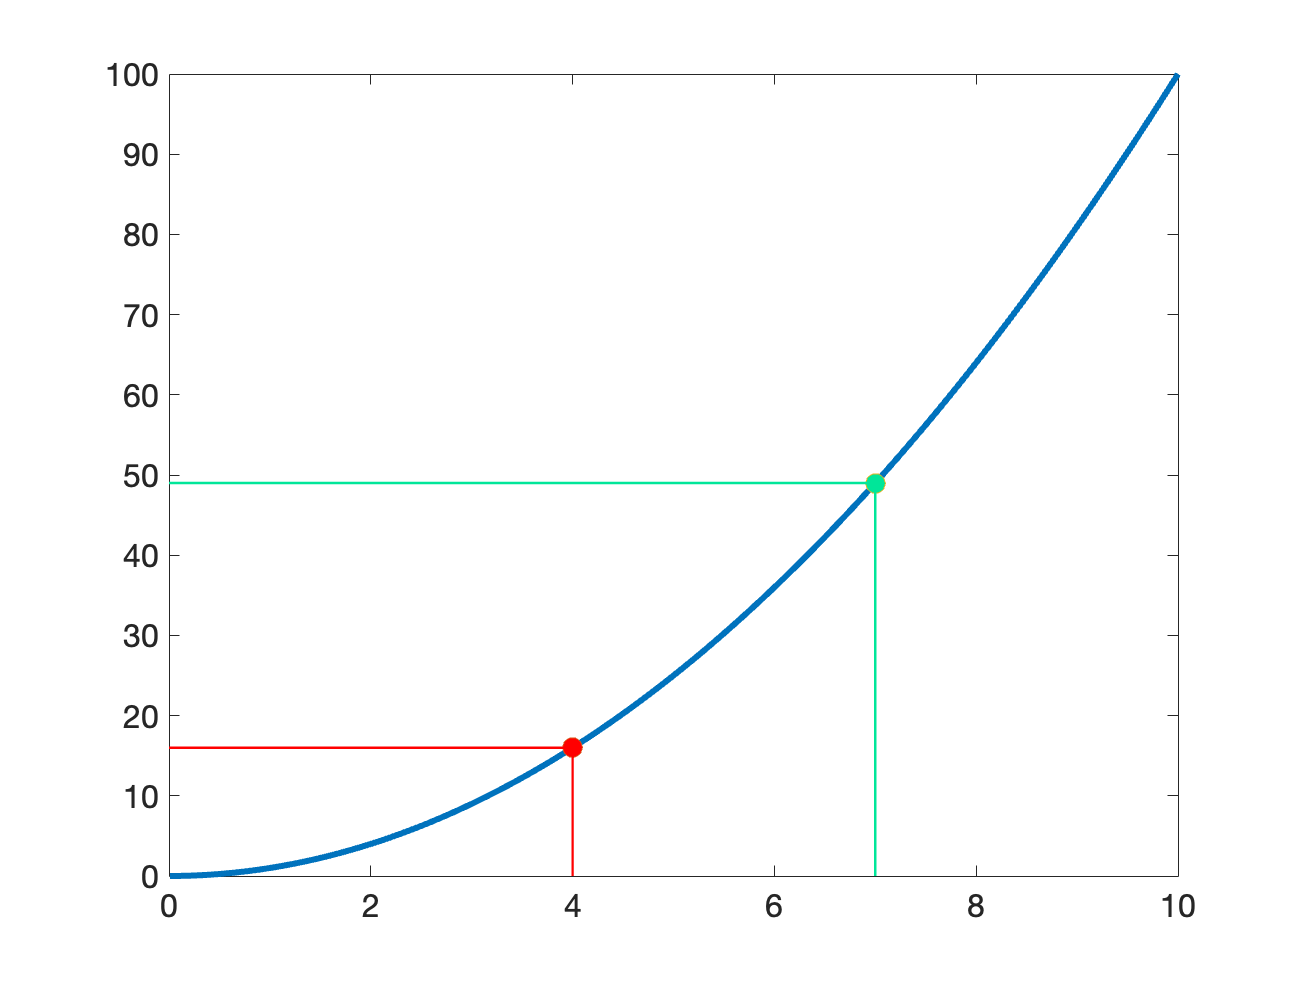
\includegraphics[width=0.85\linewidth]{example_sqrt}
			\caption{Graph of $f(x\geq 0) = x^2$; Since the function is monotonic, larger argument implies larger output.}
		\end{figure}
		
		
	\end{flushleft}
\end{frame}



\begin{frame}{Least squares at a glance (1)}
	% \framesubtitle{Parameter estimation}
	\begin{flushleft}
		
		Consider the following problem: find $\bo{x}$ that minimizes $|| \bo{A}\bo{x} - \bo{y} ||_2$. This is the \emph{least squares problem}. 
		
		\bigskip
		
		\begin{itemize}
			\item The value $\bo{e} = \bo{A}\bo{x} - \bo{y}$ is called residual.
			
			\item Least squares problem is about finding \emph{least residual solution}.
		\end{itemize}
		
		Note that $f(\bo{x}) = || \bo{A}\bo{x} - \bo{y} ||_2 = \sqrt{(\bo{A}\bo{x} - \bo{y})\T(\bo{A}\bo{x} - \bo{y})}$; as we showed earlier, we can minimize the function $g(\bo{x}) = (\bo{A}\bo{x} - \bo{y})\T(\bo{A}\bo{x} - \bo{y})$ to find the same optimal value of $\bo{x}$.
		
		
	\end{flushleft}
\end{frame}




\begin{frame}{Least squares at a glance (2)}
	% \framesubtitle{Parameter estimation}
	\begin{flushleft}
		
		We find extremum of $g(\bo{x}) = (\bo{A}\bo{x} - \bo{y})\T(\bo{A}\bo{x} - \bo{y})$:
		%
		\begin{equation}
			\frac{d}{d \bo{x}} \left( 
			\textcolor{myred}{(\bo{A}\bo{x} - \bo{y})}^\top
			\textcolor{myblue}{(\bo{A}\bo{x} - \bo{y}) }
			\right) 
			= 0
		\end{equation}
		\begin{equation}
			(\bo{A}\T \textcolor{myblue}{(\bo{A}\bo{x} - \bo{y}) } )\T + 
			\textcolor{myred}{(\bo{A}\bo{x} - \bo{y})}^\top\bo{A}
			= 0
		\end{equation}
		\begin{equation}
			2\bo{A}^\top(\bo{A}\bo{x} - \bo{y}) = 0
		\end{equation}
		\begin{equation}
			\bo{A}^\top\bo{A}\bo{x} = \bo{A}^\top\bo{y}
		\end{equation}
		\begin{equation}
			\bo{x} = (\bo{A}^\top\bo{A})^{-1} \bo{A}^\top\bo{y}
		\end{equation}
		
		Thus we can define a \emph{pseudoinverse}:
		%
		\begin{equation}
			\bo{A}^+ = (\bo{A}^\top\bo{A})^{-1} \bo{A}^\top
		\end{equation}
		
		
	\end{flushleft}
\end{frame}



\begin{frame}{Pseudoinverse}
	% \framesubtitle{Parameter estimation}
	\begin{flushleft}
		
		Thus the least residual solution to $\bo{A}\bo{x} = \bo{y}$ is written as:
		
		\begin{equation}
			\bo{x} = \bo{A}^+\bo{y}
		\end{equation}
		
		We already showed that it is the least-residual solution, later we will prove that it is also the \emph{smallest norm} solution (out of all solutions with the same residual).
		
	\end{flushleft}
\end{frame}




\begin{frame}{Pseudoinverse - orthonormal matrix}
% \framesubtitle{Orthonormal case}
	\begin{flushleft}
		
		Let matrix $\bo{M}$ be orthonormal (not necessarily square), meaning $\bo{M}\T \bo{M} = \bo{I}$. Its  pseudoinverse can be simplified:
		
		\begin{align}
			\bo{M}^+ = (\bo{M}^\top\bo{M})^{-1} \bo{M}^\top = \bo{M}^\top
		\end{align}
	
		\bigskip
	
		Then least squares solution to the equation $\bo{M} \bo{x} = \bo{y}$ can be found as:
		%
		\begin{align}
			\bo{x}_{LS} = \bo{M}^\top \bo{y}
		\end{align}
	
		If $\bo{M}$ is orthonormal and square, then $\bo{M}\T = \bo{M}^{-1}$.
	
	
	\end{flushleft}
\end{frame}




\begin{frame}{Computing the residual}
	% \framesubtitle{Parameter estimation}
	\begin{flushleft}
		
		Given an equation $\bo{A}\bo{x} = \bo{y}$ and least squares solution $\bo{x}_{LS} = \bo{A}^+\bo{y}$, let us compute the residual $\bo{e} = \bo{y} - \bo{A}\bo{x}_{LS}$. We substitute the solution:
		 
		\begin{equation}
			\bo{e} = \bo{y} - \bo{A}\bo{A}^+\bo{y}
		\end{equation}
		
		We observe that:
		
		\begin{itemize}
			\item The residual can be found as $\bo{e} = (\bo{I} - \bo{A}\bo{A}^+)\bo{y}$.
			
			\item The closest $\bo{A}\bo{x}$ can get to $\bo{y}$ is $\bo{y}^* = \bo{A}\bo{A}^+\bo{y}$.
			
			\item Later we will find that $\bo{A}\bo{A}^+\bo{y}$ is a \emph{projection} of $\bo{y}$ onto a \emph{column space} of $\bo{A}$.
		\end{itemize}
		
	\end{flushleft}
\end{frame}





\begin{frame}{Four Fundamental Subspaces}
	% \framesubtitle{Parameter estimation}
	\begin{flushleft}
		
		One of the key ideas in Linear Algebra is that every linear operator has four fundamental subspaces:
		
		\begin{itemize}
			\item Null space
			\item Row space
			\item Column space
			\item Left null space
		\end{itemize}
		
		\bigskip
		
		Our goal is to understand them. The usefulness of this concept is enormous.
		
	\end{flushleft}
\end{frame}

\begin{frame}{Null space}
	\framesubtitle{Definition}
	\begin{flushleft}
		
		Consider the following task: find all solutions to the system of equations $\mathbf{A} \mathbf{x} = \mathbf{0}$.
		
		\bigskip
		
		It can be re-formulated as follows: find all elements of the \emph{null space} of $\mathbf{A}$.
		
		\begin{block}{Definition 1}
			\emph{Null space} of $\mathbf{A}$ is the set of all vectors $\mathbf{x}$ that $\mathbf{A}$ maps to $\mathbf{0}$
		\end{block}
		
		\bigskip
		
		We will denote null space as $\textcolor{mydarkgray}{\text{null}(\mathbf{A})}$. Null space of an operator is sometimes called \emph{kernel} and denoted as $\textcolor{mydarkgray}{\text{ker}(\mathbf{A})}$.
		
	\end{flushleft}
\end{frame}


\begin{frame}{Null space}
	\framesubtitle{Calculation}
	\begin{flushleft}
		
		We can find all solutions of the system of equations $\mathbf{A} \mathbf{x} = \mathbf{0}$ by using functions that generate an \emph{orthonormal basis} in the null space of $\mathbf{A}$. In MATLAB we can use the function \texttt{null}, in Python/Scipy - \texttt{null\_space}:
		
		\bigskip
		
		\begin{itemize}
			\item \texttt{N = null(A)}.
			\item \texttt{N = scipy.linalg.null\_space(A)}.
		\end{itemize}
		
		
	\end{flushleft}
\end{frame}



\begin{frame}{Null space projection}
	\framesubtitle{Local coordinates}
	\begin{flushleft}
		
		Let $\bo{N}$ be the orthonormal basis in the null space of matrix $\bo{A}$. Then, if a vector $\bo{x}$ lies in the null space of $\bo{A}$, it can be represented as:
		
		\begin{equation}
			\bo{x} = \bo{N}\bo{z}
		\end{equation}
		%
		where $\bo{z}$ are coordinates of $\bo{x}$ in the basis $\bo{N}$.
		
		\bigskip
		
		However, there are vectors which not only are not lying in the null space of $\bo{A}$,  but the closest vector to them in the null space is the zero vector.
		
	\end{flushleft}
\end{frame}


\begin{frame}{Closest element from a linear subspace}
	% \framesubtitle{Orthogonality, examples}
	\begin{flushleft}
		
		$\bo{A} = \begin{bmatrix} 0 & 1 \\ 0 & 0\end{bmatrix}$. Its null space has orthonormal basis $\bo{N} = \begin{bmatrix} 1 \\ 0\end{bmatrix}$. 
		
		\begin{itemize}
			\item $\begin{bmatrix} -2 \\ 0 \end{bmatrix} = 
			-2 \bo{N}$,
			$\begin{bmatrix} 10 \\ 0 \end{bmatrix} = 
			10 \bo{N}$, - both are in the null space.
			\item for $\bo{x} = \begin{bmatrix} 1 \\ 1 \end{bmatrix}$ the closest vector in the null space is $\begin{bmatrix} 1 \\ 0 \end{bmatrix}$.
			\item for $\bo{y} = \begin{bmatrix} 0 \\ 2 \end{bmatrix}$ the closest vector in the null space is $\begin{bmatrix} 0 \\ 0 \end{bmatrix}$.
		\end{itemize}
		
		
	\end{flushleft}
\end{frame}



\begin{frame}{Orthogonality, definition (1)}
	% \framesubtitle{Orthogonality, definition}
	\begin{flushleft}
		
		\begin{definition}
			Any two vectors, $\bo{x}$ and $\bo{y}$, whose dot product is zero are said to be \emph{orthogonal} to each other.
		\end{definition}
		
		\begin{definition}
			Vector $\bo{y}$, whose dot product with any $\bo{x} \in \mathcal{L}$ is zero is orthogonal to the subspace $\mathcal{L}$
		\end{definition}
		
		\begin{definition}[equivalent, see Appendix A]
			If for a vector $\bo{y}$, the closest vector to it from a linear subspace $\mathcal{L}$ is zero vector, $\bo{y}$ is called orthogonal to the subspace $\mathcal{L}$.
		\end{definition}
		
		
	\end{flushleft}
\end{frame}


\begin{frame}{Orthogonality, definition (2)}
	% \framesubtitle{Orthogonality, definition}
	\begin{flushleft}
		
		\begin{definition}
			The space of all vectors $\bo{y}$, orthogonal to a linear subspace $\mathcal{L}$ is called \emph{orthogonal complement} of $\mathcal{L}$ and is denoted as $\mathcal{L}^\perp$.
		\end{definition}
		
		
		\begin{definition}[equivalent]
			The space of all vectors $\bo{y}$, such that $\text{dot}(\bo{y}, \bo{x}) = 0$, $\forall \bo{x} \in \mathcal{L}$ is called \emph{orthogonal complement} of $\mathcal{L}$.
		\end{definition}
		
		Therefore $\bo{x} \in \mathcal{L}$ and $\bo{y} \in \mathcal{L}^\perp$ implies $\text{dot}(\bo{y}, \bo{x}) = 0$.
		
	\end{flushleft}
\end{frame}





\begin{frame}{Projection, 1}
	\begin{flushleft}
		
		Let $\bo{L}$ be an orthonormal basis in a linear subspace $\mathcal{L}$. Take vector $\bo{a} = \bo{x} + \bo{y}$, where $\bo{x}$ lies in the subspace $\mathcal{L}$, and $\bo{y}$ lies in the subspace $\mathcal{L}^\perp$.
		
		\bigskip
		
		\begin{definition}
			We call such vector $\bo{x}$ an \emph{orthogonal projection} of $\bo{a}$ onto subspace $\mathcal{L}$, and such vector $\bo{y}$ an orthogonal projection of $\bo{a}$ onto subspace $\mathcal{L}^\perp$
		\end{definition}
		
		\bigskip
		
		Orthogonal projection maps a vector to the element in the subspace closest to that vector. Orthogonal projection of $\bo{a}$ onto $\mathcal{L}$ can be found as: 
		
		\begin{equation}
			\bo{x} = \bo{L} \bo{L}^+ \bo{a}
		\end{equation}
		
		Since $\bo{L}$ is orthonormal, this is the same as $\bo{x} = \bo{L} \bo{L}^\top \bo{a}$
		
	\end{flushleft}
\end{frame}



\begin{frame}{Projection, 2}
	\begin{flushleft}
		
		Since $\bo{a} = \bo{x} + \bo{y}$, and $\bo{x} = \bo{L} \bo{L}^+ \bo{a}$, we can write:
		
		\begin{equation}
			\bo{a} = \bo{L} \bo{L}^+ \bo{a} + \bo{y}
		\end{equation}
		%
		from which it follows that the projection of $\bo{a}$ onto $\mathcal{L}^\perp$ can be found as: 
		
		\begin{equation}
			\bo{y} = (\bo{I} - \bo{L} \bo{L}^+) \bo{a}
		\end{equation}
		%
		where $\bo{I}$ is an identity matrix. Since $\bo{L}$ is orthonormal, this is the same as $\bo{y} = (\bo{I} - \bo{L} \bo{L}^\top) \bo{a}$
		
	\end{flushleft}
\end{frame}




\begin{frame}{Row space}
	\begin{flushleft}
		
		\begin{definition}
			Let $\mathcal{N}$ be null space of $\bo{A}$. Then orthogonal complement $\mathcal{N}^\perp$ is called \emph{row space} of $\bo{A}$.
		\end{definition}
	
		\bigskip
		
		Row space of $\bo{A}$ is the space of all smallest-norm solutions of $\bo{A}\bo{x} = \bo{y}$, for $\forall \bo{y}$. We will denote row space as $\textcolor{mydarkgray}{\text{row}(\bo{A})}$.
		
	\end{flushleft}
\end{frame}




\begin{frame}{Vectors in Null and Row spaces}
	\begin{flushleft}
		
		Given vector $\bo{x}$, matrix $\bo{A}$ and its null space basis $\bo{N}$, we check if $\bo{x}$ is in the null space of $\bo{A}$. The simplest way is to check if $\bo{A}\bo{x} = 0$. But sometimes we may want to avoid computing $\bo{A}\bo{x}$, for example if the number of elements of $\bo{A}$ is much larger than the number of elements of $\bo{N}$.
		
		\bigskip
		
		If $\bo{x}$ is in the null space of $\bo{A}$, it will have zero projection onto the row space of $\bo{A}$. This gives us the condition we can check:
		
		\begin{equation}
			(\bo{I} - \bo{N} \bo{N}^\top) \bo{x} = 0
		\end{equation}
		
		By the same logic, condition for being in the row space is as follows:
		
		\begin{equation}
			\bo{N} \bo{N}^\top \bo{x} = 0
		\end{equation}
		
		
	\end{flushleft}
\end{frame}



\begin{frame}{Column space}
	\begin{flushleft}
		
		Given a matrix $\bo{A}$ find all linear combinations of its columns: $\mathcal{C} = \{ \bo{y}: \ \bo{y} = \bo{A} \bo{x}, \ \forall \bo{x}  \}$.
		
		\bigskip
		
		It can be re-formulated as follows: find all elements of the \emph{column space} of $\bo{A}$.
		
		\begin{block}{Definition - column space}
			\emph{Column space} of $\bo{A}$ is the set of all outputs of the matrix $\bo{A}$, for all possible inputs.
		\end{block}
		
		\bigskip
		
		We will denote column space as $\textcolor{mydarkgray}{\text{col}(\bo{A})}$. It is often called an \emph{image} of $\bo{A}$.
		
		
	\end{flushleft}
\end{frame}



\begin{frame}{Column space basis}
	\begin{flushleft}
		
		The problem of finding orthonormal basis in the column space of a matrix is often called \emph{orthonormalization} of that matrix. Hence in MATLAB and Python/Scipy the function that does it is called \texttt{orth}:
		
		\bigskip
		
		\begin{itemize}
			\item \texttt{C = orth(A)}.
			\item \texttt{C = scipy.linalg.orth(A)}.
		\end{itemize}
		
		\bigskip
		
%		That is how one finds all the outputs of the matrix $\bo{A}$: as $\{ \bo{C}\bo{z}: \ \forall \bo{z} \}$. 
%		
%		Notice that $\{ \bo{A}\bo{x}: \ \forall \bo{x} \}$ might contain repeated entries if $\bo{A}$ has a non-trivial null space.
		
	\end{flushleft}
\end{frame}



\begin{frame}{Column and null spaces}
	% \framesubtitle{Local coordinates}
	\begin{flushleft}
		
		Let $\bo{A}$ be a square matrix, a map from $\mathbb{X} = \R^n$ to $\mathbb{Y} = \R^n$. 
		Notice that if it has a non-trivial null space, it follows that multiple unique inputs are being mapped by it to the same output:
		
		\begin{equation}
			\begin{aligned}
				\bo{y} = \bo{A} \bo{x}_r = \bo{A} (\bo{x}_r + \bo{x}_n), \\
				\bo{x}_r \in \text{row}(\bo{A}) \\
				\forall \bo{x}_n \in \text{null}(\bo{A}) \\
			\end{aligned}
		\end{equation}
		
		In fact, if null space of $\bo{A}$ has $k$ dimensions, it implies that an $k$-dimensional subspace of $\mathbb{X}$ is mapped to a single element of $\mathbb{Y}$. 
		
		\bigskip
		
		It follows that in this case the dimensionality of the column space could not exceed $n-k$.
		
	\end{flushleft}
\end{frame}



\begin{frame}{Projector onto column space}
	% \framesubtitle{Local coordinates}
	\begin{flushleft}
		
		Given vector $\bo{y}$ and matrix $\bo{A}$, let us find $\bo{y}_c$ - projection of $\bo{y}$ onto the column space of $\bo{A}$.
		
		\bigskip
		
		Since $\bo{y}_c \in \text{col}(\bo{A})$, we can find such $\bo{x}$ that $\bo{A}\bo{x} = \bo{y}_c$; so, the problems is to minimize the residual $e = || \bo{y}_c - \bo{y} ||$ or equivalently $e =  || \bo{A}\bo{x} - \bo{y} ||$, which is least squares problem: $\bo{x} = \bo{A}^+ \bo{y}$. So:
		
		\begin{equation}
			\bo{y}_c = \bo{A}\bo{A}^+ \bo{y} \in \text{col}(\bo{A})
		\end{equation}
		
		Remember that computing the pseudoinverse is based on SVD decomposition, same as finding a basis in the null space or the column space, so in terms of computational expense, all projections we discussed are similar.
		
	\end{flushleft}
\end{frame}



\begin{frame}{Projector onto row space}
	% \framesubtitle{Local coordinates}
	\begin{flushleft}
		
		Similarly we can define a projector onto the row space. Given vector $\bo{x}$ and matrix $\bo{A}$, let us find projector of $\bo{x}$ onto the row space of $\bo{A}$:
		
		\begin{equation}
			\bo{x}_r = \bo{A}^+\bo{A} \bo{x} \in \text{row}(\bo{A})
		\end{equation}
		
		You can think of this in the following terms: first we find output $\bo{A} \bo{x}$, then we find the smallest norm vector that produces this same output; this vector  1) has the same row space projection (because output is the same), 2) has zero null space projection. Hence it is the row space projector of $\bo{x}$.
		
		\bigskip
		
		Notice that we implicitly used the fact that columns of $\bo{A}^+$ lie in the row space of $\bo{A}$. We will prove this fact later. Additionally, we will prove that row space of $\bo{A}$ is equivalent to the column space of $\bo{A}^\top$.
		
	\end{flushleft}
\end{frame}




\begin{frame}{Left null space}
	% \framesubtitle{Local coordinates}
	\begin{flushleft}
		
		The subspace, orthogonal to the column space is called \emph{left null space}.
		
		\bigskip
		
		\begin{definition}
			Space of all vectors $\bo{y}$ orthogonal to the columns of $\bo{A}$ is called \emph{left null space}: $\bo{y}^\top\bo{A} = 0$
		\end{definition}
		
		You can think of left null space as a space of vectors that not only cannot be produced (as an output) by the operator $\bo{A}$, but the closest vector to them that can be produced is the zero vector.
		
		\bigskip
		
		Notice that $\bo{y}\T \bo{A} = 0$ implies $\bo{A}\T \bo{y} = 0$, meaning that left null space of $\bo{A}$ is equivalent to the null space of $\bo{A}\T$.
		
		
	\end{flushleft}
\end{frame}




\begin{frame}{Left null space projector}
	% \framesubtitle{Local coordinates}
	\begin{flushleft}
		
		If we want to project vector $\bo{y}$ onto the left null space of $\bo{A}$, we project it onto the column space, and subtract the result from $\bo{y}$:
		
		\begin{equation}
			\bo{y}_l = (\bo{I} - \bo{A}\bo{A}^+) \bo{y} \in \text{left null}(\bo{A})
		\end{equation}
		
		If $\bo{C}$ is an orthonormal basis in the column space of $\bo{A}$, the projection can be found the following way:
		
		\begin{equation}
			\bo{y}_l = (\bo{I} - \bo{C}\bo{C}^\top) \bo{y} \in \text{left null}(\bo{A})
		\end{equation}
		
		
	\end{flushleft}
\end{frame}



\begin{frame}{Singular Value Decomposition}
	% \framesubtitle{Local coordinates}
	\begin{flushleft}
		
		Given $\bo{A} \in \R^{n, m}$ we can find its Singular Value Decomposition (SVD):
		
		\begin{equation}
			\bo{A} = 
			\begin{bmatrix}
				\bo{C} & \bo{L}
			\end{bmatrix}
			\begin{bmatrix}
				\bo{\Sigma} & \bo{0} \\
				\bo{0} & \bo{0}
			\end{bmatrix}
			\begin{bmatrix}
				\bo{R}^\top \\ \bo{N}^\top
			\end{bmatrix}
		\end{equation}
		
		\begin{equation}
			\bo{A} = 
			\bo{C} \bo{\Sigma} \bo{R}^\top
		\end{equation}
		
		where $\bo{C}$, $\bo{L}$, $\bo{R}$ and $\bo{N}$ are column, left null, row and null space bases (orthonormal), $\bo{\Sigma}$ is the diagonal matrix of singular values. The singular values are positive and are sorted in the decreasing order.
		
		\bigskip

		Rank of the matrix is computed as the size of $\bo{\Sigma}$. Note that numeric tolerance applies when deciding if the singular value is non-zero.
		
	\end{flushleft}
\end{frame}




\begin{frame}{SVD of a transpose}
	% \framesubtitle{Local coordinates}
	\begin{flushleft}
		
		Let us find SVD decomposition of a $\bo{A}^\top$:
		
		\begin{equation}
			\bo{A}^\top = 
			\begin{bmatrix}
				\bo{C}_t & \bo{L}_t
			\end{bmatrix}
			\begin{bmatrix}
				\bo{\Sigma}_t & \bo{0} \\
				\bo{0} & \bo{0}
			\end{bmatrix}
			\begin{bmatrix}
				\bo{R}_t^\top \\ \bo{N}_t^\top
			\end{bmatrix}
		\end{equation}
		
		Let us transpose it (remembering that transpose of a diagonal matrix the original matrix $\bo{\Sigma}_t^\top = \bo{\Sigma}_t$):
		
		
		\begin{equation}
			\bo{A} = 
			\begin{bmatrix}
				\bo{R}_t & \bo{N}_t
			\end{bmatrix}
			\begin{bmatrix}
				\bo{\Sigma}_t & \bo{0} \\
				\bo{0} & \bo{0}
			\end{bmatrix}
			\begin{bmatrix}
				\bo{C}_t^\top \\ \bo{L}_t^\top
			\end{bmatrix}
		\end{equation}
		
		Thus we can see that the row space of the original matrix $\bo{A}$ is the column space of the transpose $\bo{A}^\top$. And the left null space of the original matrix $\bo{A}$ is the null space of the transpose $\bo{A}^\top$.
		
		
	\end{flushleft}
\end{frame}



\begin{frame}{Pseudoinverse via SVD, 1}
	% \framesubtitle{Local coordinates}
	\begin{flushleft}
		
		Let us compute least squares - minimum of $e = ||\bo{A}\bo{x} - \bo{y}||_2$. We find extremum:
		%
		\begin{align}
			\frac{d}{d \bo{x}} \left( (\bo{A}\bo{x} - \bo{y})^\top(\bo{A}\bo{x} - \bo{y}) \right) 
			= 0
			\\
			2\bo{A}^\top(\bo{A}\bo{x} - \bo{y}) = 0
			\\
			\bo{A}^\top\bo{A}\bo{x} = \bo{A}^\top\bo{y}
		\end{align}
		
		We find SVD decomposition of $\bo{A} = \bo{C} \bo{\Sigma} \bo{R}^\top$:
		%
		\begin{align}
			\bo{R}  \bo{\Sigma} \bo{C}\T   \bo{C} \bo{\Sigma} \bo{R}^\top \bo{x} = \bo{R}  \bo{\Sigma} \bo{C}\T  \bo{y}
			\\
			\bo{R}  \bo{\Sigma} \bo{\Sigma} \bo{R}^\top \bo{x} = \bo{R}  \bo{\Sigma} \bo{C}\T  \bo{y}
		\end{align}
		
	\end{flushleft}
\end{frame}





\begin{frame}{Pseudoinverse via SVD, 2}
	% \framesubtitle{Local coordinates}
	\begin{flushleft}
		
		Since both sides lie in the column space of $\bo{R}$, we can multiply by $\bo{R}\T$:
		%
		\begin{align}
			\bo{R}\T\bo{R}  \bo{\Sigma} \bo{\Sigma} \bo{R}^\top \bo{x} = \bo{R}\T\bo{R}  \bo{\Sigma} \bo{C}\T  \bo{y}
			\\
			\bo{\Sigma} \bo{\Sigma} \bo{R}^\top \bo{x} = \bo{\Sigma} \bo{C}\T  \bo{y}
			\\
			\bo{R}^\top \bo{x} = \bo{\Sigma}^{-1} \bo{C}\T  \bo{y}
		\end{align}
		
		Since $\bo{R}$ and $\bo{N}$ are orthogonal compliments, we can represent $\bo{x}$ as its decomposition: $\bo{x} = \bo{N}\bo{z} + \bo{R}\zeta$:
		%
		\begin{align}
			\bo{R}^\top \bo{N}\bo{z} + \bo{R}^\top \bo{R}\zeta = \bo{\Sigma}^{-1} \bo{C}\T  \bo{y}
			\\
			\zeta = \bo{\Sigma}^{-1} \bo{C}\T  \bo{y}
		\end{align}
	
		With that we can compute $\bo{x}$:
		%
		\begin{align}
			\bo{x} = \bo{N}\bo{z} + \bo{R}\bo{\Sigma}^{-1} \bo{C}\T  \bo{y}
		\end{align}
		
	\end{flushleft}
\end{frame}



\begin{frame}{Pseudoinverse via SVD, 3}
	% \framesubtitle{Local coordinates}
	\begin{flushleft}
		
		Expression $\bo{x} = \bo{N}\bo{z} + \bo{R}\bo{\Sigma}^{-1} \bo{C}\T  \bo{y}$ gives us all least-residual solutions.
		
		\bigskip
		
		Since $\bo{N}\bo{z}$ is orthogonal to $\bo{R}\bo{\Sigma}^{-1} \bo{C}\T  \bo{y}$, we conclude that least-norm solution is given as:
		%
		\begin{align}
			\bo{x} = \bo{R}\bo{\Sigma}^{-1} \bo{C}\T  \bo{y}
		\end{align}
		
		With that we can define pseudoinverse matrix $\bo{A}^+$ as:
		
		\begin{equation}
			\bo{A}^+ = 
			\bo{R} \bo{\Sigma}^{-1} \bo{C}^\top
		\end{equation}		
		
		Note that this proves that $\bo{A}^+$ lies in the row space of $\bo{A}$.
		
	\end{flushleft}
\end{frame}








\begin{frame}{Projectors (1)}
	% \framesubtitle{Local coordinates}
	\begin{flushleft}
		
		Let us prove that $\bo{A}\bo{A}^+$ is equivalent to $\bo{C}\bo{C}^\top$:
		
		\begin{equation}
			\bo{A} \bo{A}^+ = 
			\bo{C} \bo{\Sigma} \bo{R}^\top 
			\bo{R} \bo{\Sigma}^{-1} \bo{C}^\top
		\end{equation}
		
		
		\begin{equation}
			\bo{A} \bo{A}^+ = 
			\bo{C} \bo{\Sigma} \bo{\Sigma}^{-1} \bo{C}^\top
		\end{equation}
		
		\begin{equation}
			\bo{A} \bo{A}^+ = 
			\bo{C} \bo{C}^\top
		\end{equation}
		
		
	\end{flushleft}
\end{frame}



\begin{frame}{Projectors (2)}
	% \framesubtitle{Local coordinates}
	\begin{flushleft}
		
		Let us prove that $\bo{A}^+\bo{A}$ is equivalent to $\bo{R}\bo{R}^\top$:
		
		\begin{equation}
			\bo{A}^+ \bo{A} = 
			\bo{R} \bo{\Sigma}^{-1} \bo{C}^\top
			\bo{C} \bo{\Sigma} \bo{R}^\top 
		\end{equation}
		
		\begin{equation}
			\bo{A}^+ \bo{A} = 
			\bo{R} \bo{\Sigma}^{-1} \bo{\Sigma} \bo{R}^\top 
		\end{equation}		
		
		\begin{equation}
			\bo{A}^+ \bo{A} = 
			\bo{R} \bo{R}^\top 
		\end{equation}			
		
	\end{flushleft}
\end{frame}





\begin{frame}{Projectors (3)}
	% \framesubtitle{Local coordinates}
	\begin{flushleft}
		
		Let us denote $\bo{P} = \bo{A}\bo{A}^+$. 
		Let's prove that $\bo{P}\bo{P} = \bo{P}$:
		
		\begin{align}
			\bo{A} \bo{A}^+ \bo{A} \bo{A}^+ &= 
			\bo{C} \bo{\Sigma} \bo{R}^\top 
			\bo{R} \bo{\Sigma}^{-1} \bo{C}^\top 
			\bo{C} \bo{\Sigma} \bo{R}^\top 
			\bo{R} \bo{\Sigma}^{-1} \bo{C}^\top
			\\
			%
			\bo{A} \bo{A}^+ \bo{A} \bo{A}^+ &= 
			\bo{C} \bo{\Sigma} \bo{\Sigma}^{-1}\bo{\Sigma} \bo{\Sigma}^{-1} \bo{C}^\top
			\\
			%
			\bo{A} \bo{A}^+ \bo{A} \bo{A}^+ &= 
			\bo{C} \bo{C}^\top
			\\
			%
			\bo{A} \bo{A}^+ \bo{A} \bo{A}^+ &= 
			\bo{A} \bo{A}^+
		\end{align}
		
		
		The same is true for $\bo{P} = \bo{A}^+\bo{A}$: we can prove that $\bo{A}^+\bo{A} \bo{A}^+\bo{A} = \bo{A}^+\bo{A}$.
		
	\end{flushleft}
\end{frame}



\begin{frame}{Transpose of a projector}
	% \framesubtitle{Local coordinates}
	\begin{flushleft}
		
		Let's prove that $\bo{P}\T = \bo{P}$. 
		
		Again, we use the fact that $\bo{P} = \bo{C}\bo{C}\T$.
		
		\begin{align}
			\bo{P}\T = (\bo{C}\bo{C}\T)\T=\bo{C}\bo{C}\T=\bo{P}. \qed
		\end{align}
		
		
	\end{flushleft}
\end{frame}



\begin{frame}{Pseudoinverse of a projector}
	% \framesubtitle{Local coordinates}
	\begin{flushleft}
		
		Let's prove that $\bo{P}^+ = \bo{P}$. 
		
		\bigskip
		
		First, we find a basis in the linear space where $\bo{P}$ projects onto: $\bo{C} = \text{col}(\bo{P})$, therefore $\bo{P} = \bo{C}\bo{C}\T = \bo{C}\bo{I}\bo{C}\T$, which is an SVD decomposition of $\bo{P}$. But we know how to find a pseudoinverse of a linear operator, given its SVD decomposition:
		%
		\begin{align}
			\bo{P} &= \bo{C}\bo{I}\bo{C}\T,
			\\
			\bo{P}^+ &= \bo{C}\bo{I}^{-1}\bo{C}\T,
			\\
			\bo{P}^+ &= \bo{C}\bo{C}\T,
			\\
			\bo{P}^+ &= \bo{P}. \ \qed
		\end{align}
		
		
	\end{flushleft}
\end{frame}




\begin{frame}{Further reading}
	% \framesubtitle{Local coordinates}
	\begin{flushleft}
		
		\begin{itemize}
			\item \bref{https://faculty.math.illinois.edu/~mlavrov/docs/484-spring-2019/ch4lec4.pdf}{Minimum Norm Solutions, Math 484: Nonlinear Programming, Mikhail Lavrov}
			%https://faculty.math.illinois.edu/~mlavrov/courses/484-spring-2019.html
			
			\item \bref{https://faculty.math.illinois.edu/~mlavrov/docs/484-spring-2019/ch4lec3.pdf}{Orthogonality, Math 484: Nonlinear Programming, Mikhail Lavrov}
			
			\item \bref{http://databookuw.com/databook.pdf}{Data Driven Science \& Engineering. Machine Learning, Dynamical Systems, and Control, Steven L. Brunton, J. Nathan Kutz}, chapter Singular Value Decomposition (SVD)
			
		\end{itemize}
		
		
	\end{flushleft}
\end{frame}




\begin{frame}{Exercise}
	% \framesubtitle{Local coordinates}
	\begin{flushleft}
		
		\begin{itemize}
			\item Matrix $\bo{M}$ is orthonormal and square, prove that $\bo{M}\T = \bo{M}^{-1}$.
			
			\item Find minimum of $||\bo{A}\bo{x} - \bo{y}||_2$ when columns of $\bo{A}$ are not linearly independent.
			
			\item Given an equation $\bo{A}\bo{x} = \bo{y}$ with a square matrix $\bo{A}$, prove that: either that equation has an exact solution for any $\bo{y}$ or a related homogeneous equation $\bo{A}\bo{x} = 0$ has a non-trivial solution.
		\end{itemize}
		
		
		
	\end{flushleft}
\end{frame}




\myqrframe



\begin{frame}{Appendix A}
	% \framesubtitle{Local coordinates}
	\begin{flushleft}
		
		We have two definitions of orthogonality of a vector and a subspace:
		
		\begin{enumerate}
			\item Vector $\bo{y}$, whose dot product with any $\bo{x} \in \mathcal{L}$ is orthogonal to the subspace $\mathcal{L}$
			
			\item If for a vector $\bo{y}$, the closest vector to it from a linear subspace $\mathcal{L}$ is zero vector, $\bo{y}$ is called orthogonal to the subspace $\mathcal{L}$.
		\end{enumerate}
		
	Let us prove their equivalence. First we show that 1) implies 2). Let $\bo{L}$ be orthonormal basis in $\mathcal{L}$. To find the closest element $\bo{y}^*$ of $\mathcal{L}$ to $\bo{y}$, we need to solve the least squares problem $\bo{L}\bo{z} = \bo{y}$, and multiply the solution by $\bo{L}$:
	
	\begin{align}
		\bo{z}_{LS} &= \bo{L}\T \bo{y} = \bo{0} \\
    	\bo{y}^* = \bo{L}\bo{z}_{LS} &= \bo{L}\bo{L}\T \bo{y} = \bo{0}
	\end{align}		
		
	\end{flushleft}
\end{frame}


\begin{frame}{Appendix A}
	% \framesubtitle{Local coordinates}
	\begin{flushleft}
		
		
		Second, let us prove that 2) implies 1). Given that $\bo{y}^* = \bo{L}\bo{z}_{LS} = \bo{L}\bo{L}\T \bo{y} = \bo{0}$ we need to prove that $\bo{L}\T \bo{y} = \bo{0}$. We start by multiplying the last equation by $\bo{L}\T$:
		
		\begin{align}
			& \bo{L}\bo{L}\T \bo{y} = \bo{0} \\
			& \bo{L}\T \bo{L}\bo{L}\T \bo{y} = \bo{0} \\
			& \bo{L}\T \bo{y} = \bo{0}  \ \ \ \ \ \ \textcolor{mygray}{\text{since }  \bo{L}\T \bo{L} = \bo{I}}. \ \qed
		\end{align}		
		
	\end{flushleft}
\end{frame}





\end{document}
